% Copyright (c) 2013 Joost van Zwieten
%
% Permission is hereby granted, free of charge, to any person obtaining a copy
% of this software and associated documentation files (the "Software"), to deal
% in the Software without restriction, including without limitation the rights
% to use, copy, modify, merge, publish, distribute, sublicense, and/or sell
% copies of the Software, and to permit persons to whom the Software is
% furnished to do so, subject to the following conditions:
%
% The above copyright notice and this permission notice shall be included in
% all copies or substantial portions of the Software.
%
% THE SOFTWARE IS PROVIDED "AS IS", WITHOUT WARRANTY OF ANY KIND, EXPRESS OR
% IMPLIED, INCLUDING BUT NOT LIMITED TO THE WARRANTIES OF MERCHANTABILITY,
% FITNESS FOR A PARTICULAR PURPOSE AND NONINFRINGEMENT. IN NO EVENT SHALL THE
% AUTHORS OR COPYRIGHT HOLDERS BE LIABLE FOR ANY CLAIM, DAMAGES OR OTHER
% LIABILITY, WHETHER IN AN ACTION OF CONTRACT, TORT OR OTHERWISE, ARISING FROM,
% OUT OF OR IN CONNECTION WITH THE SOFTWARE OR THE USE OR OTHER DEALINGS IN
% THE SOFTWARE.
%
\documentclass{tudelftposter}

% optional, makes QR code clickable
\usepackage[hidelinks,implicit=false,bookmarks=false]{hyperref}

\title{Building complete free and open source GIS infrastructure for
  hydrological computing and data publication using GIS.lab and
  Gisquick platforms}

\addauthornote{mail}[@]{\ttfamily martin.landa@fsv.cvut.cz}
\addauthornote{diam}{Faculty of Civil Engineering, CTU in Prague}
\addauthornote{tp}[**]{OpenGeoLabs s.r.o., Czech Republic}

\addauthor[mail,diam]{M. Landa}
\addauthor[diam]{P. Kavka}
\addauthor[diam]{L. Strouhal}
\addauthor[tp]{J. Cepicky}

\addfootimage(c:right column.center)[Czech Technical University in Prague]{cvut}
\addfootqrcode(l:left column.left)[Derived from latex-poster-class]{https://github.com/tudelft-diam-na/latex-poster-class}

\begin{document}

\section{Introduction}

Building a complete open source GIS infrastructure allowing operations
from data preparation, analysis and computation to publishing results
to end-user is a very complex task. There are two major conditions for
creating well organized, and fully operational open source
infrastructure: (a) solid bricks and (b) flexible glue to integrate
them. Solid bricks represent a mature, well-driven open source GIS
software projects. Crucial factor is the integration layer which puts
all components together in a flexible but solid
manner. Underestimating the importance of such integration layer
(glue) leads to various problems in the infrastructure maintanance,
with upgrading or replacing bricks (software packages), and hardware
equipment.

This poster presents GIS.lab as an open source software solution which
helps to build such complete fully open source GIS infrastructure in
an easy, but still fully customized manner.

\section{GIS.lab as a Core Component}

\begin{figure}[ht!]
\begin{center}
  \includegraphics[width=.30\columnwidth]{../paper/figures/gislab-logo.png}
  \caption{GIS.lab logo (source: GIS.lab Documentation)}
\label{fig:gislab_logo}
\end{center}
\end{figure}

GIS.lab (\url{http://web.gislab.io}) has been originally designed with
a goal to enable simple, unbreakable deployment of a complete,
centrally managed, horizontally scalable GIS infrastructure in the
local network area (LAN), data center or cloud in a few steps. GIS.lab
is able to turn diverse open source GIS software packages into a
seamlessly integrated easy-to-use system. As a result GIS.lab
significantly decreases deployment of such complex GIS infrastructure
to absolute minimum, but still keeping the whole technology under a
full control of the system operator. 

\section{Gisquick as a Publication Platform}

Gisquick (\url{http://gisquick.org}) is a separate project not
directly related to GIS.lab. It is a web application based on modern
technologies as Django, Angular and OpenLayers 3 with fully responsive
design optimized also for mobile devices. The main purpose of Gisquick
is to provide the capability for easy publishing the QGIS projects on
the web. From this perspective Gisquick is strongly connected to QGIS
Desktop environment and stands on QGIS Server component.

% KAO: Remove spacing before label: can cause reference to be wrong
\begin{figure}[ht!]
\begin{center}
  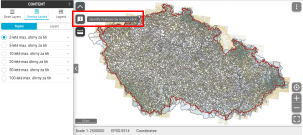
\includegraphics[width=0.9\columnwidth]{../paper/figures/gisquick-identify.png}
  \caption{Gisquick web application interface
    (source: author)}
\label{fig:gislab_infrastructure}
\end{center}
\end{figure}

Combining GIS.lab and Gisquick technologies leads to a complete, seamlessly
integrated platform capable to prepare the input data, perform geospatial
analysis and publish results easily on the web in the sense of interactive
web mapping application.

\section{Conclusions}

Geospatial cluster can be arranged thanks to open source orchestration
technologies in an automated and easily maintainable manner. GIS.lab
significantly reduces the whole procedure of design, deployment and
configuration of GIS infrastructure to the virtual minimum. GIS.lab
itself offers basic components, tools, and services for building GIS
(and not only GIS) infrastructure. GIS cluster consists of the master
node and the client nodes.

The master and client nodes can be customized using the specific
Ansible Playbooks including software provisioning and configuration
management. Integration of the new components can be simplified by the
Docker containers in order to combine them into the working system
seamlessly integrated into the customized infrastructure.

\end{document}
% vim: tw=80:ts=2:sts=2:sw=2:et:fdm=marker:fmr=[[[,]]]
